% Options for packages loaded elsewhere
\PassOptionsToPackage{unicode}{hyperref}
\PassOptionsToPackage{hyphens}{url}
%
\documentclass[
  a4paper,
]{article}
\usepackage{amsmath,amssymb}
\usepackage{setspace}
\usepackage{iftex}
\ifPDFTeX
  \usepackage[T1]{fontenc}
  \usepackage[utf8]{inputenc}
  \usepackage{textcomp} % provide euro and other symbols
\else % if luatex or xetex
  \usepackage{unicode-math} % this also loads fontspec
  \defaultfontfeatures{Scale=MatchLowercase}
  \defaultfontfeatures[\rmfamily]{Ligatures=TeX,Scale=1}
\fi
\usepackage{lmodern}
\ifPDFTeX\else
  % xetex/luatex font selection
\fi
% Use upquote if available, for straight quotes in verbatim environments
\IfFileExists{upquote.sty}{\usepackage{upquote}}{}
\IfFileExists{microtype.sty}{% use microtype if available
  \usepackage[]{microtype}
  \UseMicrotypeSet[protrusion]{basicmath} % disable protrusion for tt fonts
}{}
\makeatletter
\@ifundefined{KOMAClassName}{% if non-KOMA class
  \IfFileExists{parskip.sty}{%
    \usepackage{parskip}
  }{% else
    \setlength{\parindent}{0pt}
    \setlength{\parskip}{6pt plus 2pt minus 1pt}}
}{% if KOMA class
  \KOMAoptions{parskip=half}}
\makeatother
\usepackage{xcolor}
\usepackage[margin=1in]{geometry}
\usepackage{color}
\usepackage{fancyvrb}
\newcommand{\VerbBar}{|}
\newcommand{\VERB}{\Verb[commandchars=\\\{\}]}
\DefineVerbatimEnvironment{Highlighting}{Verbatim}{commandchars=\\\{\}}
% Add ',fontsize=\small' for more characters per line
\usepackage{framed}
\definecolor{shadecolor}{RGB}{248,248,248}
\newenvironment{Shaded}{\begin{snugshade}}{\end{snugshade}}
\newcommand{\AlertTok}[1]{\textcolor[rgb]{0.94,0.16,0.16}{#1}}
\newcommand{\AnnotationTok}[1]{\textcolor[rgb]{0.56,0.35,0.01}{\textbf{\textit{#1}}}}
\newcommand{\AttributeTok}[1]{\textcolor[rgb]{0.13,0.29,0.53}{#1}}
\newcommand{\BaseNTok}[1]{\textcolor[rgb]{0.00,0.00,0.81}{#1}}
\newcommand{\BuiltInTok}[1]{#1}
\newcommand{\CharTok}[1]{\textcolor[rgb]{0.31,0.60,0.02}{#1}}
\newcommand{\CommentTok}[1]{\textcolor[rgb]{0.56,0.35,0.01}{\textit{#1}}}
\newcommand{\CommentVarTok}[1]{\textcolor[rgb]{0.56,0.35,0.01}{\textbf{\textit{#1}}}}
\newcommand{\ConstantTok}[1]{\textcolor[rgb]{0.56,0.35,0.01}{#1}}
\newcommand{\ControlFlowTok}[1]{\textcolor[rgb]{0.13,0.29,0.53}{\textbf{#1}}}
\newcommand{\DataTypeTok}[1]{\textcolor[rgb]{0.13,0.29,0.53}{#1}}
\newcommand{\DecValTok}[1]{\textcolor[rgb]{0.00,0.00,0.81}{#1}}
\newcommand{\DocumentationTok}[1]{\textcolor[rgb]{0.56,0.35,0.01}{\textbf{\textit{#1}}}}
\newcommand{\ErrorTok}[1]{\textcolor[rgb]{0.64,0.00,0.00}{\textbf{#1}}}
\newcommand{\ExtensionTok}[1]{#1}
\newcommand{\FloatTok}[1]{\textcolor[rgb]{0.00,0.00,0.81}{#1}}
\newcommand{\FunctionTok}[1]{\textcolor[rgb]{0.13,0.29,0.53}{\textbf{#1}}}
\newcommand{\ImportTok}[1]{#1}
\newcommand{\InformationTok}[1]{\textcolor[rgb]{0.56,0.35,0.01}{\textbf{\textit{#1}}}}
\newcommand{\KeywordTok}[1]{\textcolor[rgb]{0.13,0.29,0.53}{\textbf{#1}}}
\newcommand{\NormalTok}[1]{#1}
\newcommand{\OperatorTok}[1]{\textcolor[rgb]{0.81,0.36,0.00}{\textbf{#1}}}
\newcommand{\OtherTok}[1]{\textcolor[rgb]{0.56,0.35,0.01}{#1}}
\newcommand{\PreprocessorTok}[1]{\textcolor[rgb]{0.56,0.35,0.01}{\textit{#1}}}
\newcommand{\RegionMarkerTok}[1]{#1}
\newcommand{\SpecialCharTok}[1]{\textcolor[rgb]{0.81,0.36,0.00}{\textbf{#1}}}
\newcommand{\SpecialStringTok}[1]{\textcolor[rgb]{0.31,0.60,0.02}{#1}}
\newcommand{\StringTok}[1]{\textcolor[rgb]{0.31,0.60,0.02}{#1}}
\newcommand{\VariableTok}[1]{\textcolor[rgb]{0.00,0.00,0.00}{#1}}
\newcommand{\VerbatimStringTok}[1]{\textcolor[rgb]{0.31,0.60,0.02}{#1}}
\newcommand{\WarningTok}[1]{\textcolor[rgb]{0.56,0.35,0.01}{\textbf{\textit{#1}}}}
\usepackage{longtable,booktabs,array}
\usepackage{calc} % for calculating minipage widths
% Correct order of tables after \paragraph or \subparagraph
\usepackage{etoolbox}
\makeatletter
\patchcmd\longtable{\par}{\if@noskipsec\mbox{}\fi\par}{}{}
\makeatother
% Allow footnotes in longtable head/foot
\IfFileExists{footnotehyper.sty}{\usepackage{footnotehyper}}{\usepackage{footnote}}
\makesavenoteenv{longtable}
\usepackage{graphicx}
\makeatletter
\def\maxwidth{\ifdim\Gin@nat@width>\linewidth\linewidth\else\Gin@nat@width\fi}
\def\maxheight{\ifdim\Gin@nat@height>\textheight\textheight\else\Gin@nat@height\fi}
\makeatother
% Scale images if necessary, so that they will not overflow the page
% margins by default, and it is still possible to overwrite the defaults
% using explicit options in \includegraphics[width, height, ...]{}
\setkeys{Gin}{width=\maxwidth,height=\maxheight,keepaspectratio}
% Set default figure placement to htbp
\makeatletter
\def\fps@figure{htbp}
\makeatother
\setlength{\emergencystretch}{3em} % prevent overfull lines
\providecommand{\tightlist}{%
  \setlength{\itemsep}{0pt}\setlength{\parskip}{0pt}}
\setcounter{secnumdepth}{-\maxdimen} % remove section numbering
\ifLuaTeX
  \usepackage{selnolig}  % disable illegal ligatures
\fi
\usepackage{bookmark}
\IfFileExists{xurl.sty}{\usepackage{xurl}}{} % add URL line breaks if available
\urlstyle{same}
\hypersetup{
  pdftitle={U4. WINDOWS SERVER. ADMINISTRACIÓ I CONFIGURACIÓ},
  hidelinks,
  pdfcreator={LaTeX via pandoc}}

\title{U4. WINDOWS SERVER. ADMINISTRACIÓ I CONFIGURACIÓ}
\usepackage{etoolbox}
\makeatletter
\providecommand{\subtitle}[1]{% add subtitle to \maketitle
  \apptocmd{\@title}{\par {\large #1 \par}}{}{}
}
\makeatother
\subtitle{QUOTES DE DISC EN WINDOWS SERVER 2019}
\author{}
\date{\vspace{-2.5em}}

\begin{document}
\maketitle

{
\setcounter{tocdepth}{2}
\tableofcontents
}
\setstretch{1.5}
\renewcommand\tablename{Tabla}
\newpage

\section{1 INTRODUCCIÓ}\label{introducciuxf3}

En xarxes amb dades compartides entre usuaris ens interessa establir
límits d'emmagatzematge per controlar un mal ús o abús dels recursos
evitant que algun usuari ocupe més espai del que, com a administradors
del domini, entenem que, necessita. Aquestes limitacions son el que en
els SO entenem per \emph{quotes}.

En aquesta unitat les estudiarem al Domini basat en Windows Server i més
avant en Linux Server.

\section{2 QUOTES EN WINDOWS SERVER}\label{quotes-en-windows-server}

Les quotes de disc realitzen un seguiment i controlen l'ús de l'espai de
disc en els volums NTFS. Quan habilites quotes de disc, pots configurar
dos valors:

\begin{itemize}
\item
  El límit de la quota de disc
\item
  El nivell d'advertència de la quota de disc.
\end{itemize}

Per exemple, pots configurar un límit de quota de disc de 100 megabytes
(MB) i un nivell d'advertència de quota de disc de 80 MB.

Evidentment l'administració de quotes en un volum requereix drets
d'administrador en el Servidor (algun software de configuració tocarem)
però també estem condicionant o limitant els drets del usuaris del
domini, per tant, haurem de ser un usuari Administrador del domini (el
grup Admins.del dominio, per exemple).

\subsection{Límit per carpetes}\label{luxedmit-per-carpetes}

Windows Server ens permet mitjançant el ROL ``Administrador de recursos
del servidor de archivos'' aplicar les quotes a carpetes individuals.
Açò combinat amb les tècniques de:

\begin{itemize}
\tightlist
\item
  Carpetes Particular
\item
  readreçament de Documents
\item
  carpetes compartides
\end{itemize}

Ens permet fer una gestió de l'espai secundari de la xarxa molt bona.

\subsection{Compressió de dades}\label{compressiuxf3-de-dades}

Amb la compressió d'arxius no eludim el control si configurem aquest en
local, ja que el seguiment es fa atenent a la seua grandària original,
sense comprimir.

Per contra, en fer un seguiment de l'ús del volum en les carpetes
compartides, Windows calcula el límit de quota mitjançant la grandària
comprimida.

\subsubsection{No interacció entre
usuaris}\label{no-interacciuxf3-entre-usuaris}

La utilització de l'espai de disc que faça cada usuari, no afectarà a
les quotes de disc d'altres usuaris del mateix volum.

Per exemple, si un usuari guarda diversos arxius amb una mida de 100
megabytes (MB) al Volum E, que té un límit de quota de 500 megabytes, no
podrà escriure més dades en el volum si no elimina o mou abans diversos
dels arxius existents. Tanmateix, la resta dels usuaris encara poden
guardar en aquest volum. Les quotes de disc es basen en \textbf{el
propietari} dels arxius indistintament dels directoris on s'ubiquen el
fitxers.

\subsection{Quotes en volumns}\label{quotes-en-volumns}

Les quotes de disc només afecten als volums i són independents de les
estructures de les carpetes dels volums i de la seua distribució en
discs físics.

Si un sol disc físic conté diversos volums i aplica quotes a tots els
volums, cada quota de volum afecta exclusivament a aquest volum. Per
exemple, si comparteix dos volums distints, com Volum E i Volum G, es fa
un seguiment independent de les quotes per als dos volums, encara que es
troben en el mateix disc físic. Si un volum abasta múltiples discs
físics, s'aplica la mateixa quota a tot l'àmbit del volum. Per exemple,
si el Volum F té un límit de quota de 500 megabytes (MB), els usuaris no
podran guardar més de 500 MB en aquest volum, independentment de si
resideix en un disc físic o abasta tres.

\section{3 OPERATIVA}\label{operativa}

\subsection{3.1 Instal·lar el Rol de Administrador de recursos del
servidor d'arxius (File Server Resource
Manager-FSRM)}\label{installar-el-rol-de-administrador-de-recursos-del-servidor-darxius-file-server-resource-manager-fsrm}

Recordem de la Unitat 1 quan parlavem de les funcions d'un SOX. La de
servir fitxer vorem que no és estrictament guardar inforamció compartida
en disc.

El \textbf{Administrador de recursos del servidor d'arxius (FSRM)} és
essencial per gestionar quotes de disc avançades.

\begin{enumerate}
\def\labelenumi{\arabic{enumi}.}
\tightlist
\item
  Des del \textbf{Administrador del servidor} (servermanager.exe)
\item
  Afegeix rols i característiques
\item
  Selecciona \textbf{Servicios de archivos y
  almacenamiento}\textgreater{}\textbf{Servicios de iSCSI y archivo}
  \textgreater{} \textbf{Administrador de recursos del sistema de
  archivos}.
\item
  Completa l'assistent i, si es demana, reinicia el servidor.
\end{enumerate}

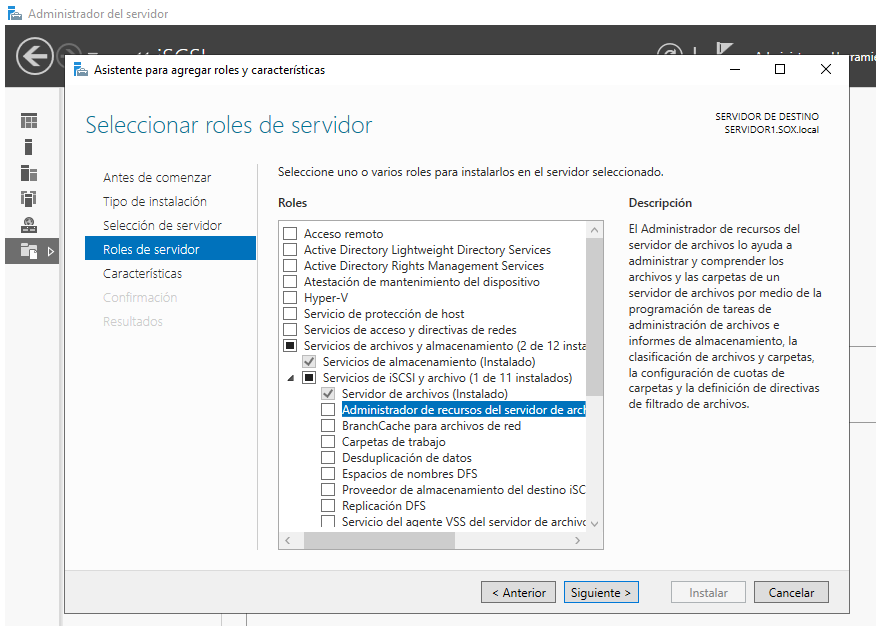
\includegraphics{png/instalaROL.png}

Opcionalment podeu fer-ho des de PowerShell (executant-lo com a
Administrador!)

\begin{Shaded}
\begin{Highlighting}[]
\NormalTok{Install{-}WindowsFeature }\OperatorTok{{-}}\NormalTok{Name FS{-}Resource{-}Manager }\OperatorTok{{-}}\NormalTok{IncludeManagementTools}
\end{Highlighting}
\end{Shaded}

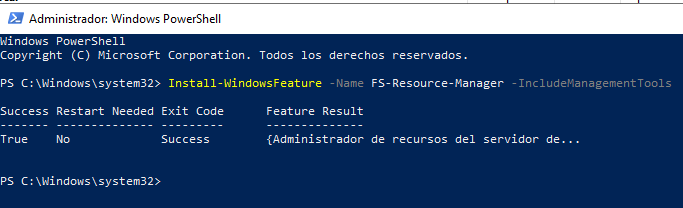
\includegraphics{png/psInstall.png}

Comprovar que el servici funciona

Podeu comprovar que el servici corresponent està Iniciat o revisar el
tipus d'inici.

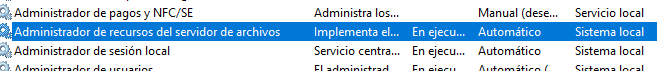
\includegraphics{png/Servici.png}

\subsection{3.2 Configura les Quotes per a les Carpetes Particulars dels
Usuaris de la Unitat
Organitzativa}\label{configura-les-quotes-per-a-les-carpetes-particulars-dels-usuaris-de-la-unitat-organitzativa}

Podem configurar per al Directori que considerem. En aquest cas anem a
usar el de les Carpetes Particulars.

Obrim l'eina i dins d'administració de quotes tenim dues opcions:

\begin{itemize}
\item
  \textbf{Quotes:} Mostra totes les quotes creades al ``Administrador de
  recursos del servidor de archivos''. Amb boto dret: \textbf{crear nova
  quota}, podrem definir una al nostre gust, ja siga partint de zero o
  utilitzant les plantilles disponibles (opció recomanada).
\item
  \textbf{Plantilles de quotes:} Mostra les plantilles existents i ens
  permet crear de noves. Podem configurar el tamany de la quota, i si
  volem que ens avise per correu electrònic o que registre un event.
\end{itemize}

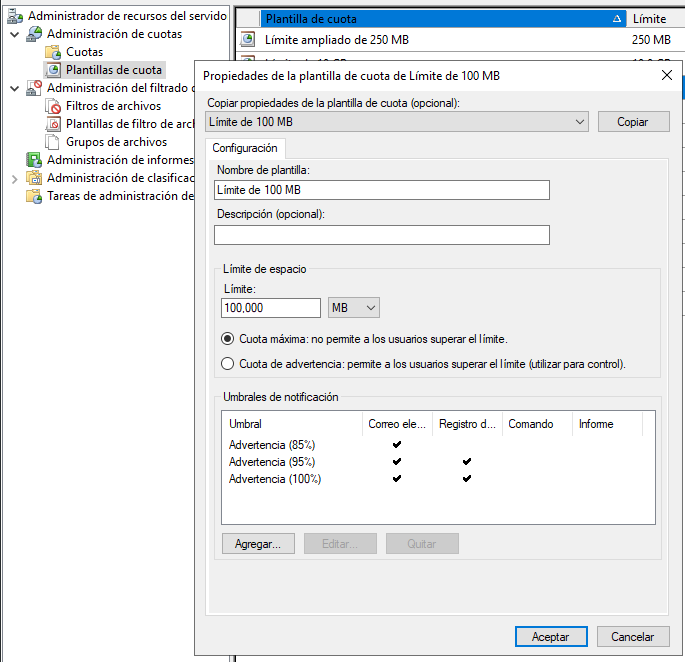
\includegraphics{png/Cuota3.png}

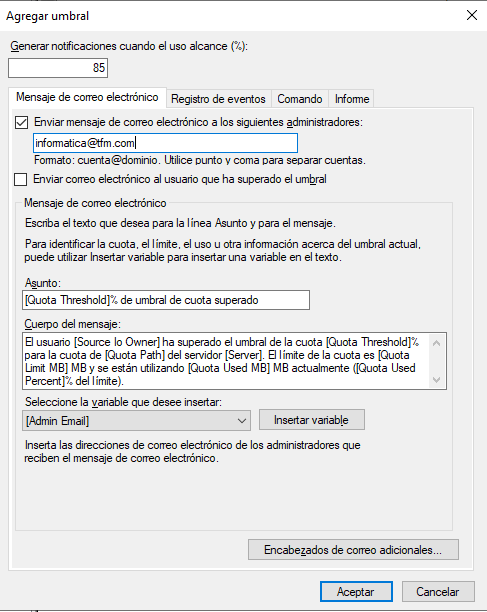
\includegraphics{png/Cuota4.png}

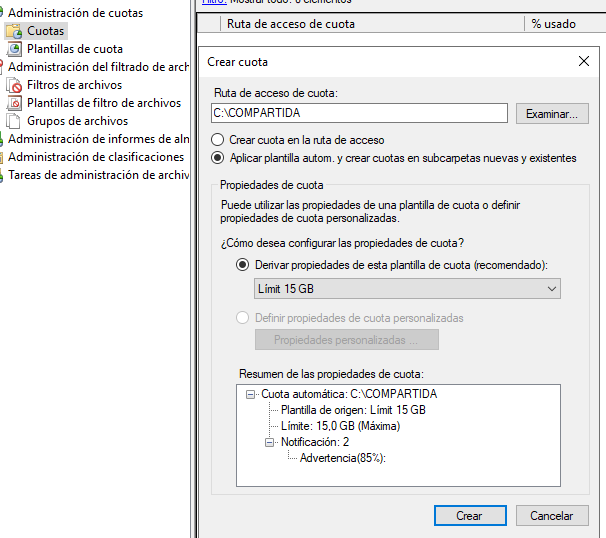
\includegraphics{png/Cuota7.png}

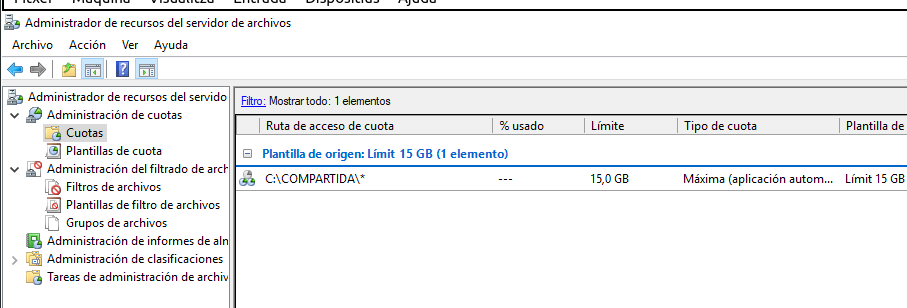
\includegraphics{png/Cuota9.png}

\subsection{Plantilles de filtre.}\label{plantilles-de-filtre.}

Al marge del tema de la limitació del tamany de disc que pot assolir una
carpeta, també podem limitar els \textbf{tipus de fitxers}que poden
guardar els usuaris.

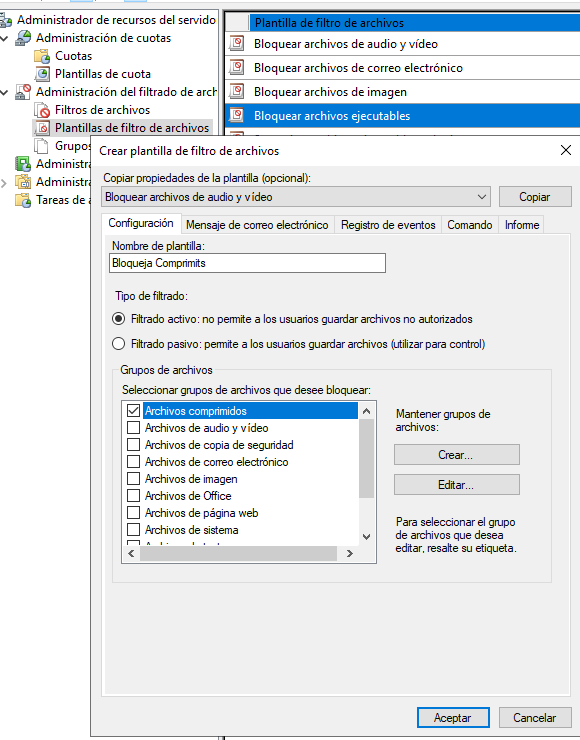
\includegraphics{png/Cuota5.png}

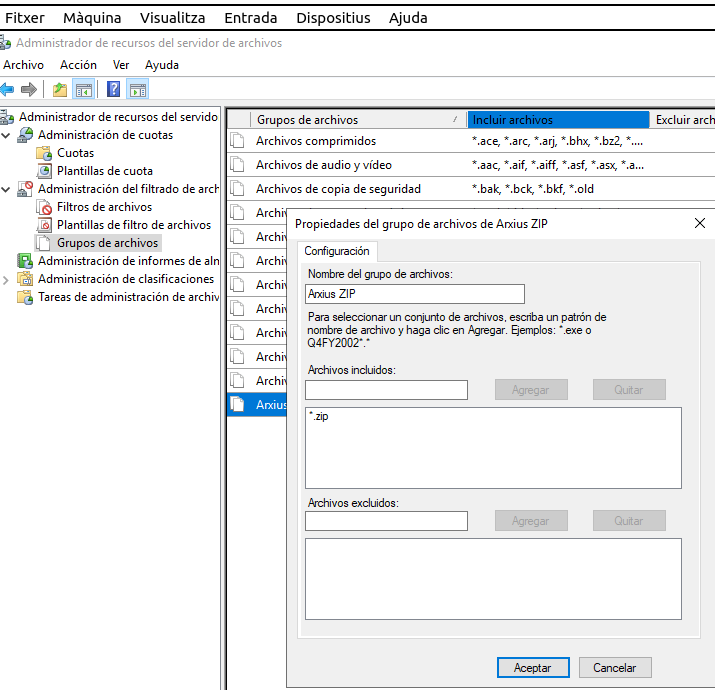
\includegraphics{png/Cuota6.png}

\subsection{L'aplicació, quan?}\label{laplicaciuxf3-quan}

L'ordre següent:

\begin{Shaded}
\begin{Highlighting}[]
\NormalTok{fsutil behavior set quotanotify 20}
\end{Highlighting}
\end{Shaded}

estableix les notificacions de quotes per avisar els usuaris cada 20
minuts sobre el seu ús de disc. Això és útil en entorns on és important
que els usuaris estiguin al corrent del seu consum d'espai per evitar
sobrepassar els límits assignats.

Per a fer proves també podem usar la mateix ordre:

\begin{Shaded}
\begin{Highlighting}[]
\NormalTok{fsutil file createnew fitxer50MB 500000000}
\end{Highlighting}
\end{Shaded}

\section{4 Diferències amb Window
1x}\label{diferuxe8ncies-amb-window-1x}

\section{Resum}\label{resum}

\begin{longtable}[]{@{}
  >{\raggedright\arraybackslash}p{(\columnwidth - 4\tabcolsep) * \real{0.2892}}
  >{\raggedright\arraybackslash}p{(\columnwidth - 4\tabcolsep) * \real{0.3614}}
  >{\raggedright\arraybackslash}p{(\columnwidth - 4\tabcolsep) * \real{0.3494}}@{}}
\toprule\noalign{}
\begin{minipage}[b]{\linewidth}\raggedright
\textbf{Nivell}
\end{minipage} & \begin{minipage}[b]{\linewidth}\raggedright
\textbf{Windows 11}
\end{minipage} & \begin{minipage}[b]{\linewidth}\raggedright
\textbf{Windows Server}
\end{minipage} \\
\midrule\noalign{}
\endhead
\bottomrule\noalign{}
\endlastfoot
\textbf{Usuari} & Sí, pots establir quotes per a cada usuari (un a un) &
Sí, pots establir quotes per a usuaris individuals. \\
\textbf{Carpeta} & No, no es poden establir quotes per carpetes. & Sí,
es poden establir quotes per a carpetes específiques. \\
\textbf{Tots els usuaris} & No, no es poden establir quotes globals per
a tots els usuaris. & Sí, pots establir quotes generals per a tots els
usuaris. \\
\textbf{Volum} & No, no es poden establir quotes per volums. & Sí, pots
establir quotes per a volums complets. \\
\textbf{Unitat} & No, no es poden establir quotes per unitats. & Sí,
pots establir quotes per unitats completes. \\
\end{longtable}

\end{document}
